\chapter{Generting Unit Tests from a UML Activity}
Our approach for automated generation of test data is based on mathematical programming and the approach for finding relevant control flow paths is based on a simple breadth first search with early infeasible path recognition. Alternatively we can also use depth first search.
%in this Chapter I am going to describe everything I Implemented in the tool as well as some Features I wanted to implement but did not have enough time for.
\section{Generel Overwiew over the Workflow}
The transformation from an UML activity to a CPP Unit test code is divided in five steps. In a first step, the Normalization, where we can check some design rules and parse all embedded OCL constraints and map only the relevant parts from the UML Model onto a simplified meta model of an Activity. The next step is the generation of a mathematical program out of our simplified test model. We are using the AMPL language for that. The third step is a path search where we can find all control flow paths or  those that are necessary to fulfil some coverage criterion of choice. In the fourth step of solving the mathematical program we need to encode a control flow path for which to generate test data in the data for our mathematical program and select a suitable solver to solve the program. In a last step we take the generated solution to the mathematical program and put the values in place within compilable and executable C++ Unit test code. An overview over the complete workflow of our approach is given in figure\ref{fig:workflowOverview}. When infeasible paths need to be detected already during the search of control flow paths the third and fourth step are interfering with each other.
\begin{figure}
\includegraphics[width=\textwidth]{pics/workflow.pdf}
\label{fig:workflowOverview}
\caption{Overview over the Unit Test generation workflow}
\end{figure}
%1.Normalize Model, 2.Make model mathematical Rigurous, 3. Search for Control flow Paths. 4 Solve Mathematical Program for the found Control flow Paths to generate specific Input and output Data. 5. Generate Unit Tests
\section{Normalisation}

\subsection{Design Rules for UML Model} %Structural Design rules
\subsubsection{structural Design Rules}
For our test generation we do assume some design rules to be applied during modelling. The Activity we generate tests from is an \UMLReference{owned Activity} of a \UMLType{Class}. The  \UMLType{Class} containing the Activity itself is contained by a \UMLType{Package} or \UMLType{Model}. 
There is an Operation specifying the Activity. This specifying Operation is either a direct sibling in the UML tree structure and has the same name as the Activity or is explicitly specified by the \UMLReference{specification} reference of the Activity.
In figure\ref{fig:StructureExample} we see a tree view of an UML model where those requirements are met.
\begin{figure}
\label{fig:StructureExample}
\includegraphics[width=\textwidht, height=0.5*\textwidth]{}
\caption{Example of a valid structured Model}
\end{figure}
\subsubsection{OCL design rules}
Further we assume that the embedded OCL constraints are either contained within a \UMLType{LiteralString} Element or an \UMLType{OpaqueExpression} with the according Language value set to "OCL". We support a strict subset of the OCL language. The BNF of the supported OCL subset is shown here.

BNF
IntegerLiteral\\
BooleanLiteral: true | false\\
RealLiteral\\
IntVariable\\
RealVariable\\
BoolVariable\\
Number: IntegerLiteral | RealLiteral | IntVariable | RealVariable | ArithmeticOperation\\
ArithmeticOpSymbol: + - * /\\
ArithmeticOperation: Number ArithmeticOpSymbol Number \\
RelationOpSymbol: < | > | <= | >= | = | <> 

RelationOperation: Number RelationOpSymbol Number \\
LogicalOpSymbol: and | or \\
LogicalOperation: Bool LogicalOpSymbol Bool \\

\subsection{A Meta Model suitable for automated Unit Test Generation}
The developed unit test generation algorithm does not work directly on an UML Model but on an ActivityTestCaseGraph. The ActivityTestCaseGraph contains only those details from the UML Metamodel that are really necessary for the test generation. Since it only contains ready parsed OCL Expressions as abstract syntax trees it is much more suitable for the transformation into a mathematical program. \\
The ActivityTestCaseGraph is defined as an extension of a more general AbstractTestCaseGraph model. The AbstractTestCaseGraph meta model was taylored to fit Activities as well as UML \UMLType{Statemachines} in order to be able to apply algorithms not only to Activities but also to \UMLType{StateMachines} as well as to be able to reuse existing Algorithms from ParTeG for \UMLType{StateMachines} for \UMLType{Activities}.

%????
%Figure \ref{fig:ATCGMetamodel} shows the complete meta model of the ActivityTestCaseGraph including all components from the AbstractTestCaseGraph.
%\begin{figure}
%\includegraphics[width=\textwidth]{./pics/ATCGMetamodel.pdf}
%\label{fig:ATCGMetamodel} 
%\caption{Complete meta model of ActivityTestCaseGraph}
%\end{figure}
%????

\subsubsection{Abstract Test Case Graph}

\begin{figure}
\label{fig:AbstractTCGMetaModel}
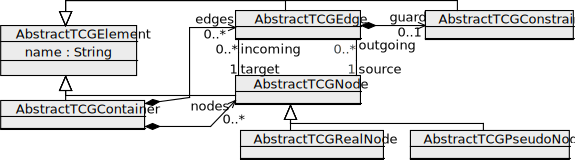
\includegraphics[width=0.5\textwidth]{./pics/AbstractTestCaseGraph.pdf}
\caption{Meta model of the AbstractTestCaseGraph}
\end{figure}
An Abstract Test Case Graph is a directed graph consisting of nodes (AbstractTCGNode) and edges (AbstractTCGEdge). Each edge has source and a target node. Each node can have multiple outgoing and multiple incoming edges.
A node can either be a pseudo node (AbstractTCGPseudoNode) or a real node (AbstractTCGRealNode). A pseudo node is a node that you can insert in the middle of an edge without changing any of the semantics of the test model. Edges can have a guard condition of type AbstractTCGConstraint. Such a graph is contained by a Container (AbstractTCGContainer). The container has a singular reference to one of its owned nodes declaring this as the initial node. \\
The semantics of the activity test case graph is Petri net like. When executing a test case graph we have at the beginning a token in the initial node that can move along the edges. The token can only move along an edge, when its guard condition is true. When an token resides in a node we say that the node is executed.

\subsubsection{Activity Test Case Graph}
\begin{figure}
\label{fig:ActivityTCGMetaModel}
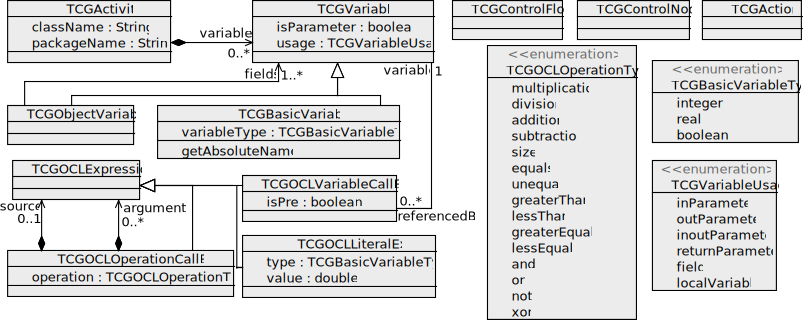
\includegraphics[width=\textwidth]{./pics/ActivityTestCaseGraph.pdf}
\caption{Meta model of the ActivityTestCaseGraph}
\end{figure}
An activity test case graph is an extension to the very simple abstract test case graph especially tailored for test generation from Activities. Its Metamodel is shown in figure\ref{fig:ActivityTCGMetaModel}.\\
The TCGActivity is an extension of the AbstractTCGContainer. As well as TCGAction, TCGControlNode and TCGControlFlow do refine the types AbstractTCGRealNode, AbstractTCGPseudoNode and AbstractTCGEdge respectively. 
The main extensions to the abstract meta model are the Variables and the elements of an abstract syntax tree to express constraints and the TCGAction.
\paragraph{TCGAction} A TCGAction can in addition to its supertye contain arbitrary many localPostconditions of the type AbstractTCGConstraint. A local Postcondition has the semantic, that it has to be true after the execution of the action. This implies changing some variables throughout the execution of the action.
\paragraph{OCL Abstract Syntax Tree}
TCGOCLExpression is a subtype of AbstractTCGConstraint. A TCGOCLexpression can either be an Operatiton call with a source and  arguments or a TCGOCLLiteralExpression holding a literal value and its data type or a TCGOCLVariableCallExp referencing a TCGVariable. The isPre attribute of TCGOCLVariableCallExp denotes whether in the original OCL expression has been an "@pre" with the token. TCGOCLExpression and its subtypes do form a simplified OCL abstract syntax tree.
\paragraph{Variables}
A TCGVariable can be one of two subtypes either a TCGBasicVariable or a TCGObjectVariable. An object variable is put together by one or more other variables. A basic variable has one of the three variableTypes that can be handled by our approach: Integer, Real, Boolean. A TCGVariable is a place holder for a value. When the isParameter field is true it can only hold one Value throughout the execution of the TCGActivity otherwise it can change its value during each execution of an TCGAction.

\subsection{Transforming UML to ActivityTestCaseGraph}
The activity test case graph serves as a normalized input model. We use a model to model transformation to transform an Activity from a UML Model into an activity test case graph. 

\subsection{Further Model 2 Model Transformations}
\subsubsection{Removing logical operations}
\subsubsection{Handling Structured Activity Nodes}
\subsubsection{Mapping self defined Datatypes to standard Types}
Explain the ActivityTestCaseGraph Metamodel and the transformation from UML with embedded OCL to it. 
suggest a few further M2M transformations to make the model easier to digest for the actual test generation.
\section{AMPL Modeling}
Tell about the AMPL Modelling i.e. variables are becoming arrays to hold one initial Value and for each TCGAction on the Path one that makes its postconditions and general Invariants valid. One specific control flow Path is encoded in the AMPL data, so we can take advantage of the interactive solving capabilities of AMPL and the connected solvers.
By adding an objective Function to the AMPL Model after any solution has been found it is extremely easy to get boundary Values for testing.
\subsection{Transforming Variables and Parameters}
\subsection{Transforming LocalPostConditions, Guards and Invariants}
\subsection{Specifying Control Flow Paths in the AMPL Data}
\subsection{Generate Boundary Values}
\section{Pathsearch}
Bounded BFS, and Bounded DFS, and DFS with early infeasible Path elimination.
Suggest to extend the search algorithms to work with test goals as explained by Stephan Weißleder.
\subsection{Depth First Search}
\subsection{Breadth First Search}
\subsection{Early Infeasible Path Elimination}
This feature can also be used to specify for loops an upper bound of iterations as well as a lower bound of loop iterations to test. You just need to add some guard conditions in front of the loop referencing the loop variant.
\section{Implementation}
say a few words about EMF and Eclipse Plugin. Tell that I used Eclipse org.eclipse.ocl.uml and eclipse org.eclipse.uml2.uml packages. //Could potentially also move to preliminaries
\subsection{The Eclipse Modelling Framework}
\cite{EMF}
\subsubsection{Importing Models from Atego Artisan Studio}
\subsubsection{Model transformations}
\subsubsection{Parsing OCL Expressions}
\subsection{Using the resulting Plugin}
